\documentclass[border=2pt]{standalone}
\usepackage{pgfplots}
\pgfplotsset{compat=1.18}
\begin{document}
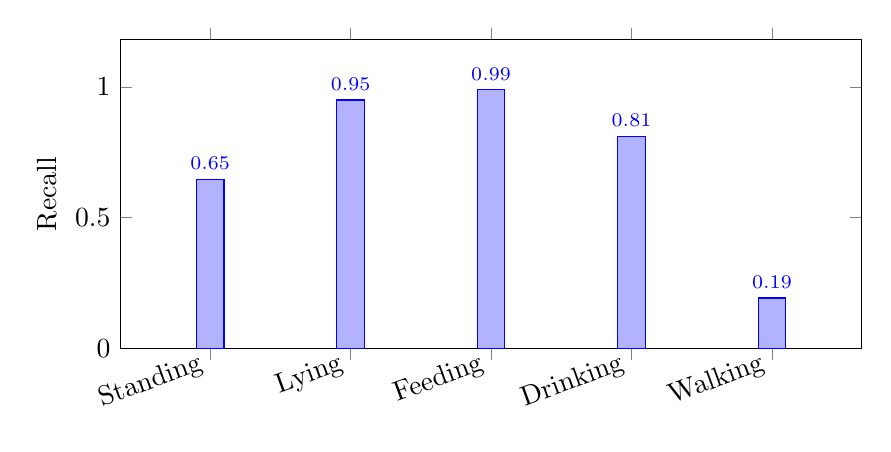
\begin{tikzpicture}
\begin{axis}[width=11cm,height=5.5cm,ybar,ymin=0,ymax=1.18,ytick={0,0.5,1.0},
 ylabel={Recall},symbolic x coords={Standing,Lying,Feeding,Drinking,Walking},
 xtick=data,x tick label style={rotate=20,anchor=east},enlarge x limits=0.16,
 nodes near coords,point meta=y,nodes near coords style={font=\scriptsize},
 /pgf/number format/fixed,/pgf/number format/precision=2]
\addplot coordinates {(Standing,0.6460) (Lying,0.9496) (Feeding,0.9885) (Drinking,0.8095) (Walking,0.1923)};
\end{axis}
\end{tikzpicture}
\end{document}